\documentclass[a4paper,12pt]{article}

\usepackage{fancyhdr}
\usepackage{lastpage}
\usepackage{amsmath}
\usepackage{tikz}
\usepackage{amsfonts}
\usepackage{graphicx}
\usepackage{float}
\usepackage{lscape}


\newcommand{\V}[1]{\ensuremath{\vec{#1}}}
\newcommand{\F}[2]{\ensuremath{\frac{#1}{#2}}}
\newcommand{\Q}[1]{\newpage \section*{#1}}
\newcommand{\acc}[1]{\overset{..}{#1}}
\newcommand{\vel}[1]{\overset{.}{#1}}
\newcommand{\prt}[2]{\frac{\partial#1}{\partial#2}}
\newcommand{\LP}{\left(}
\newcommand{\RP}{\right)}

\pagestyle{fancy}
\renewcommand{\headrulewidth}{0pt}
\fancyhf{}


\begin{document}

\begin{landscape}
  \begin{center}
    \Huge{\textbf{Monte-Carlo Soft-Sphere fluid simulation.}}\\
    \small{\textbf{Progress Report}}\\
    \Large{\textbf{Presentation by: Samuel Loomis}}\\
    \Large{\textbf{Mentor: David Roundy}}\\
      
  \end{center}
  \newpage
  \begin{figure}[h]
    \centering
    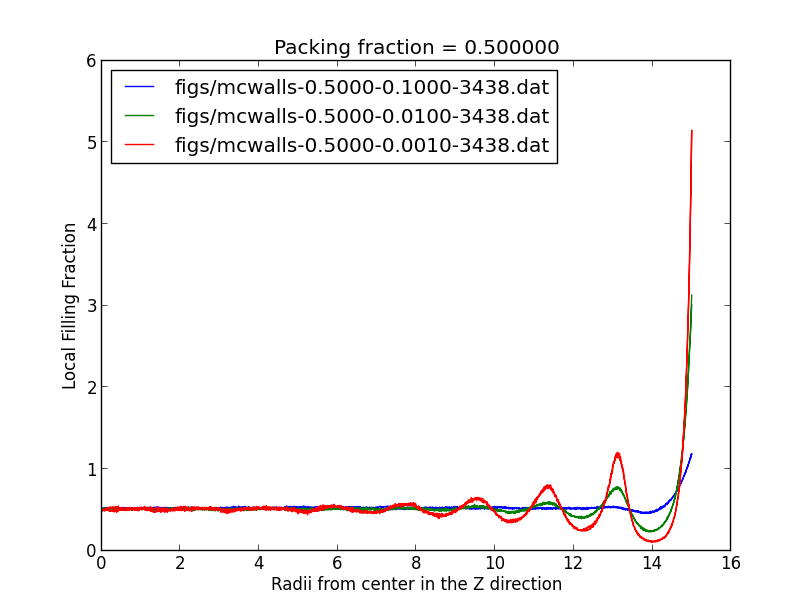
\includegraphics[width=3.75in]{full_50.png}
    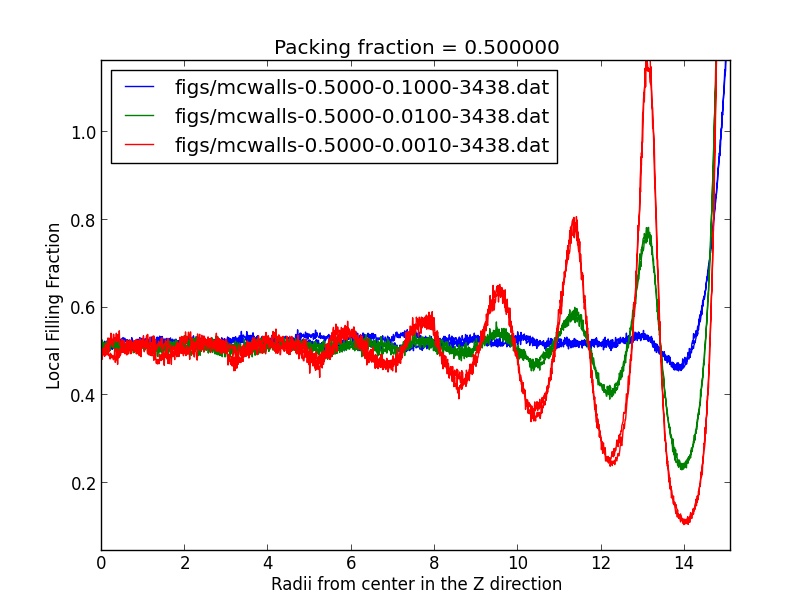
\includegraphics[width=3.75in]{bulk_50.png}
    \caption{(Left) 0.4 filling fraction Soft Sphere Monte-Carlo. (Right) Close up to observe the bulk filling fraction.}
    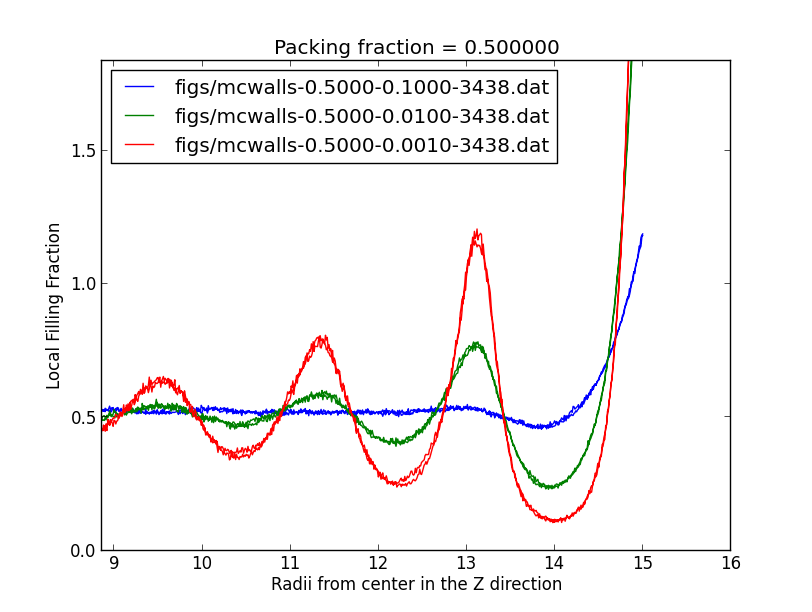
\includegraphics[width=3.75in]{wall_oscillation.png}
    \caption{Fluid wall behavior, 0.5 filling fraction.}
  \end{figure}
  \newpage
  \begin{figure}
    \centering
    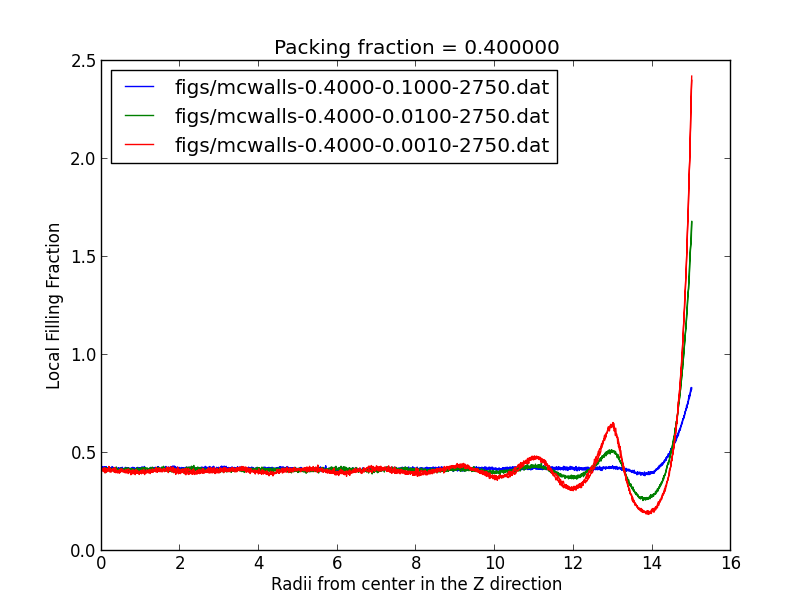
\includegraphics[width=3.75in]{full_40.png}
    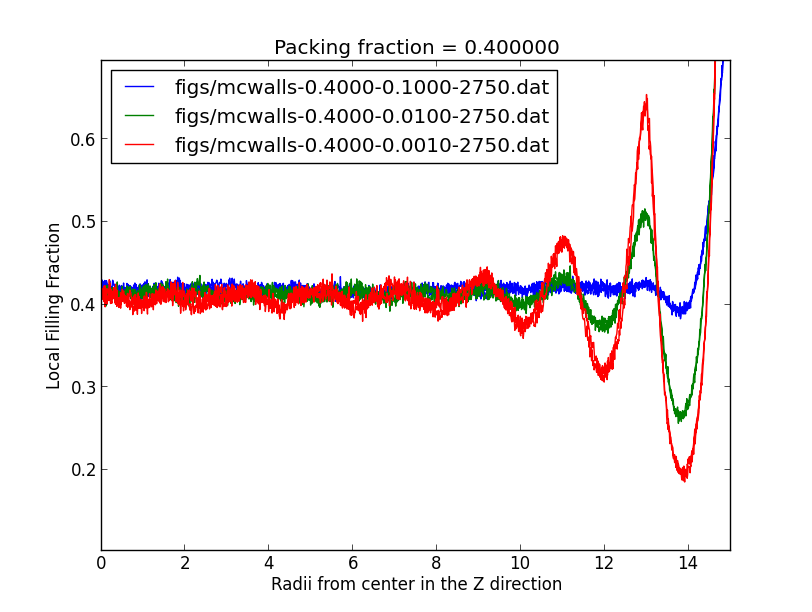
\includegraphics[width=3.75in]{bulk_40.png}
    \caption{(Left) 0.4 filling fraction Soft Sphere Monte-Carlo.  (Right) Close up to observe the bulk filling fraction.}
    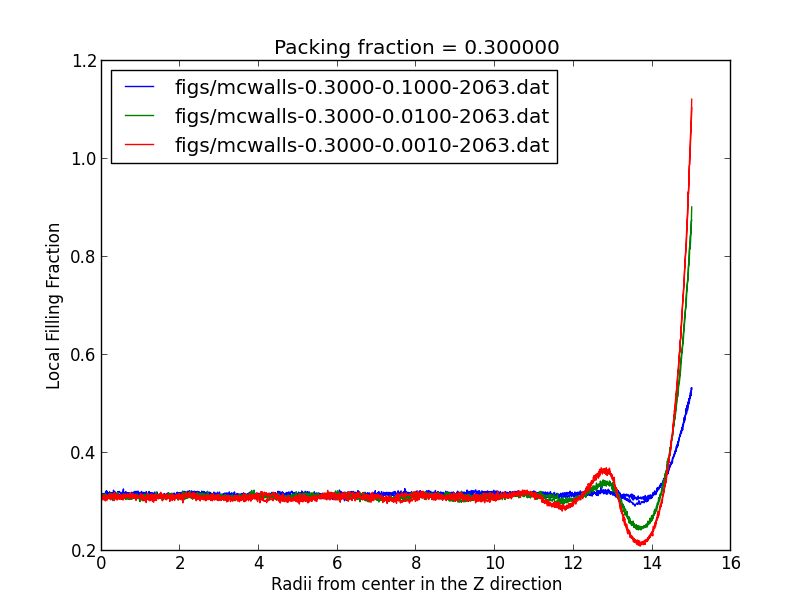
\includegraphics[width=3.75in]{full_30.png}
    \caption{0.3 filling fraction Soft Sphere Monte-Carlo.}
  \end{figure}
  \newpage
  \begin{figure}
    \centering
    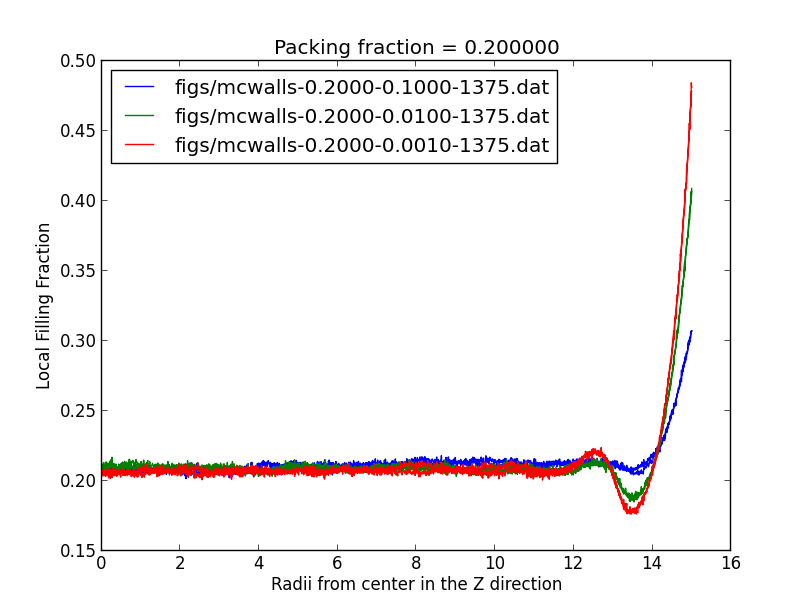
\includegraphics[width=3.75in]{full_20.png}
    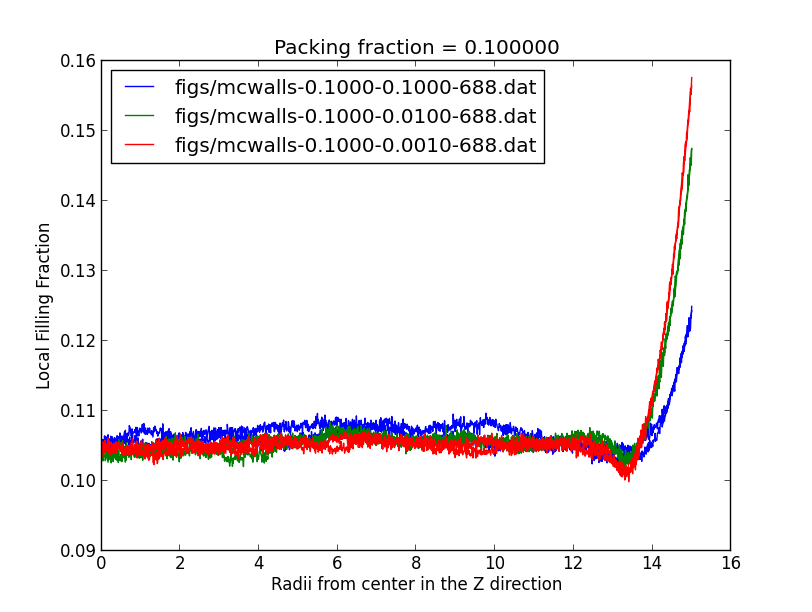
\includegraphics[width=3.75in]{full_10.png}
    \caption{(Left) 0.2 filling fraction Soft Sphere Monte-Carlo.  (Right) 0.1 filling fraction Soft Sphere Monte-Carlo.}
  \end{figure}
\end{landscape}
\end{document}
